\section{Evaluation}\label{s:evaluation}

After the detection mitigation features were implemented in HyperDbg, the effectiveness of them was tested. The evaluation of the chosen design was tested in three 
different approaches. The effectiveness of the transparency was tested against publicly available, maintained tools that compile the numerous ways hypervisors 
and debuggers can be detected into one program and executes them all one by one, as well as comparing the interception approach of Windows system calls to 
ScyllaHide~\cite{scyllahide}, an anti-anti-debugging library that applies 
a similar style of transparency to debugger detection.

The evaluation also included overhead analysis, measuring the added time overhead introduced by the transparent mitigations.

For the effectiveness evaluation, code snippets were created and implemented into small console programs that executed a specific hypervisor detection technique 
and reported the result. These were used for both overhead analysis and for the comparison with ScyllaHide, which is also designed to spoof debugger presence.

The evaluation was done on a bare metal system with an Intel CPU which supports VT-x, as well as in a nested virtualization environment running on the same bare metal system, 
where the HyperDbg hypervisor driver was deployed over a VMWare Workstation 16 virtual machine. This VM as well as the host system were running Windows 11 version 24H2 as the operating system. 
For reliability of the design, the testing was also performed on a virtual machine running Windows 11 version 24H2, 
but this was done only for reliability testing and no further evaluation measurements were taken from this system configuration. 

\subsection{Overhead Analysis}
To evaluate the performance impact of the hypervisor mitigations implemented in HyperDbg, the time overhead was measured and analyzed. 
The measurements were taken from a C++ user-space program that measured the time difference before and after executing a function that executed the evaluated hypervisor detection method. 
Each detection method was tested 20 times, and to avoid any possible caching within the process, after each measurement the program was restarted. 
These tests covered CPUID instruction querying as well as multiple system call executions. Due to the testing taking place in user-space, 
MSR reads and writes could not be tested for their overhead due to MSR access being limited to privilege ring 0~\cite[Volume 2B]{Intel-SDM2025}, and so could not be executed from user-space privilege ring.
The implementation of the mitigations involving MSR access is in a similar style to the CPUID related mitigations, so the overhead is believed to be comparable to CPUID measurements.
The time data was collected with the C++ \stress{chrono} library, 
using the \stress{high\_resolution\_clock} class\footnote{C++ chono library, high\_resolution\_clock class. \url{http://www.en.cppreference.com/w/cpp/chrono/high_resolution_clock.html}}.
All of the measurements were taken from 4 environments: a bare metal system, a bare VMWare virtual machine, and the same 
VMWare environment with the HyperDbg hypervisor deployed over it, both with and without the transparency mode enabled.

As it can be seen in Figure~\ref{fig:cpuid_exec_time} executing the CPUID instruction with the mitigations enabled, as expected, did not cause noticeable time overhead. 
This is due to the fact that mitigations for this detection method do not add any additional code to the hypervisor and other than changing the returned value, the execution path does not change.
The overhead introduced by virtualization in the execution time is discussed in section~\ref{HV_detection}.
\begin{figure}[tbh]
    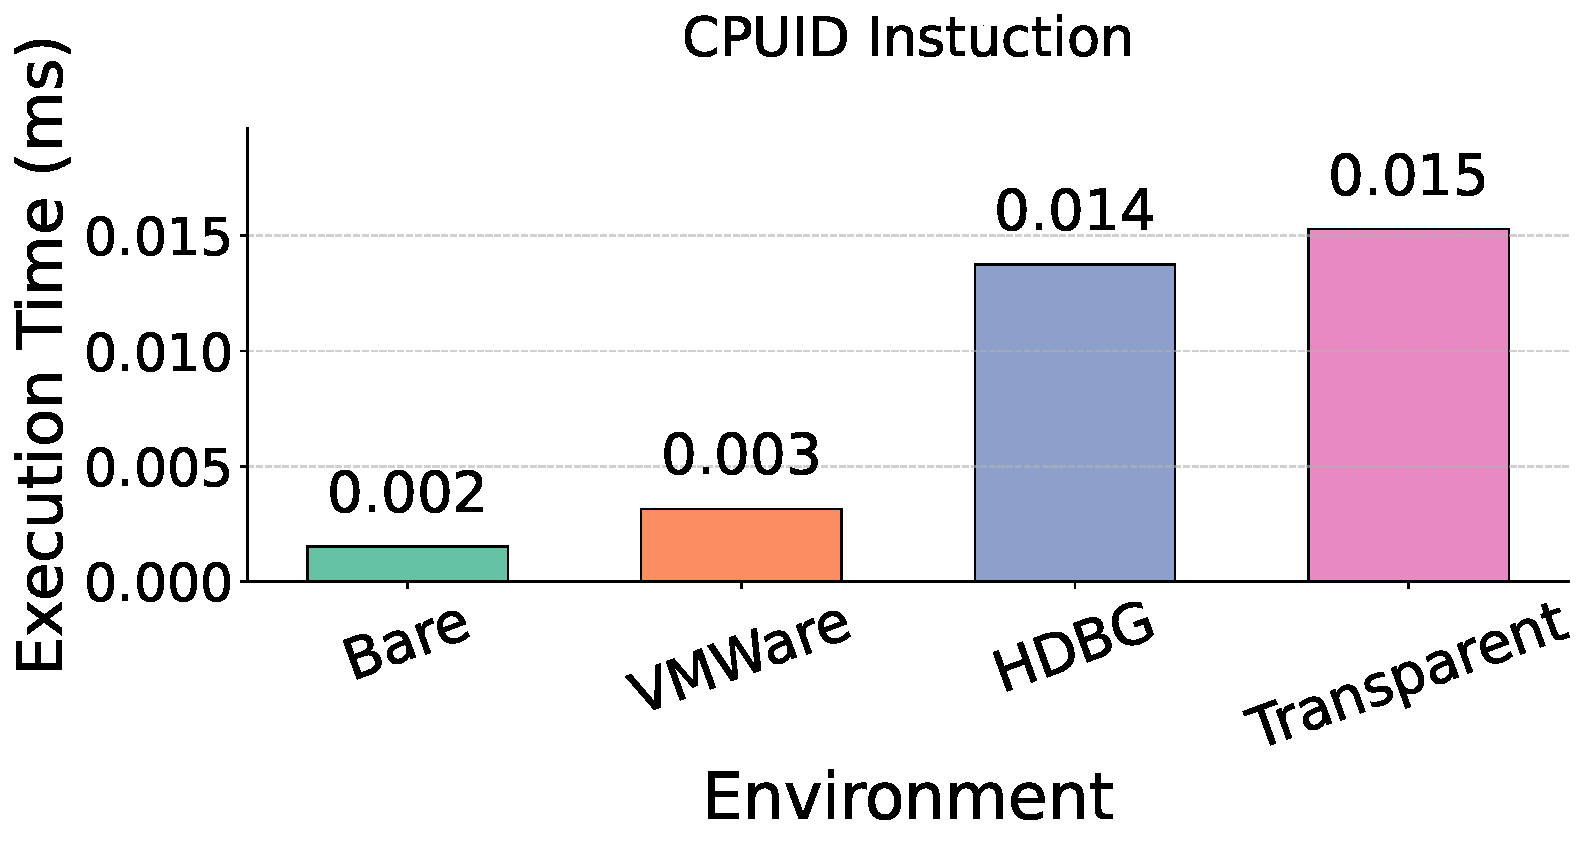
\includegraphics[width=\onecolgrid]{CPUID execution} %RDTSC_execution
    \figcap{Execution time of the CPUID instruction in different environments. HyperDbg is shortened to \stress{HDBG}, and the data for the detection mitigation transparency mode is labeled as \stress{Transparent}.}\label{fig:cpuid_exec_time}
\end{figure}

\begin{figure*}[th]
    \begin{subfigure}[t]{\threecolgrid}
        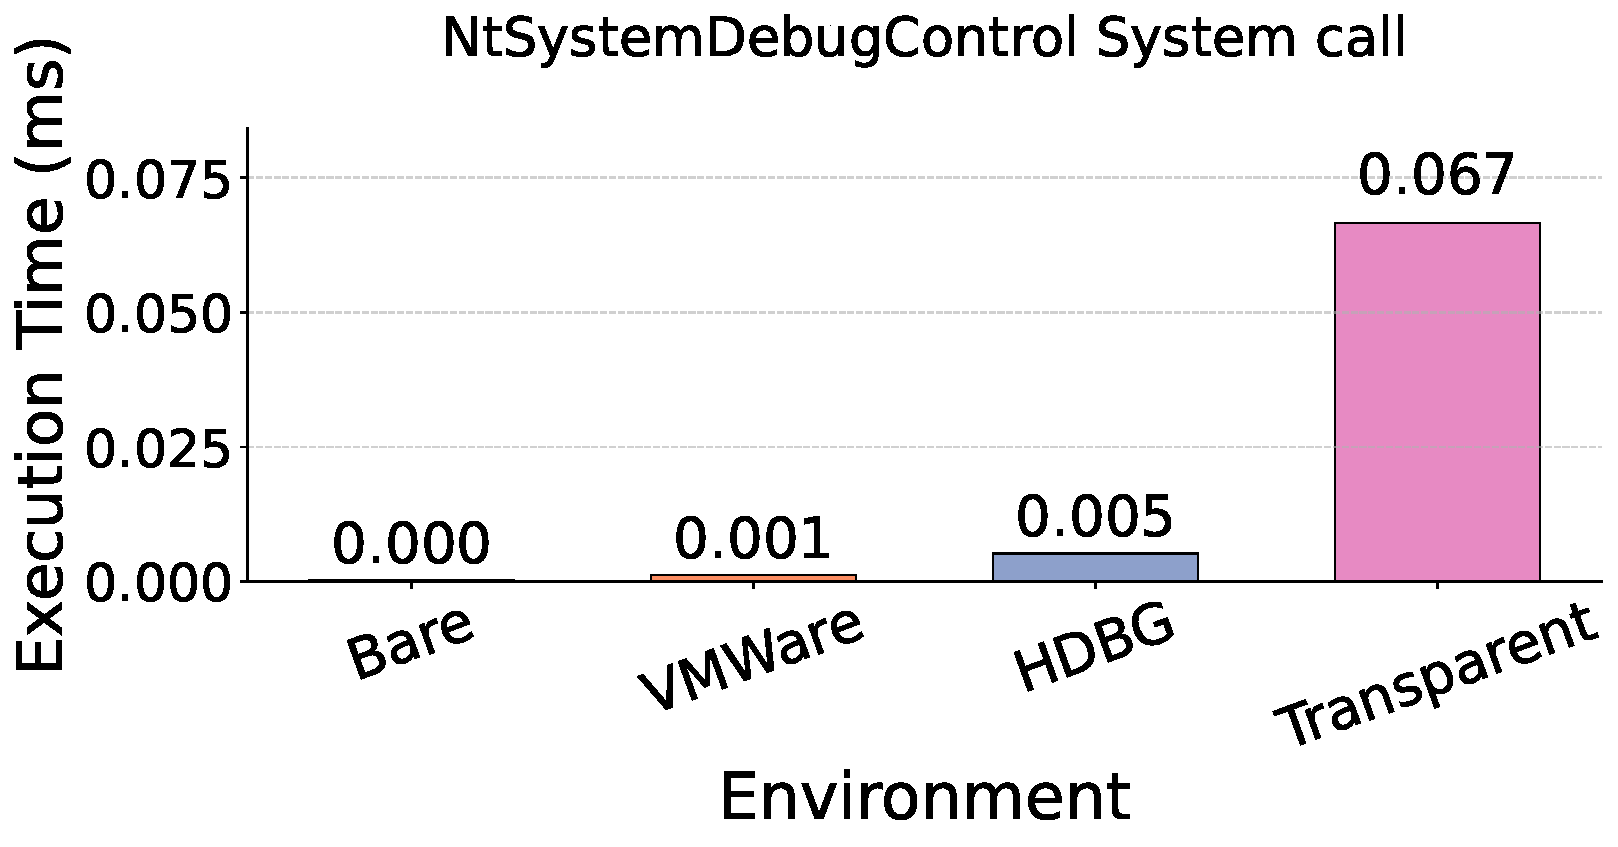
\includegraphics[width=\linewidth]{SDC execution}
        \sfigcap{}\label{fig:exec-time-a}
    \end{subfigure}
    \begin{subfigure}[t]{\threecolgrid}
        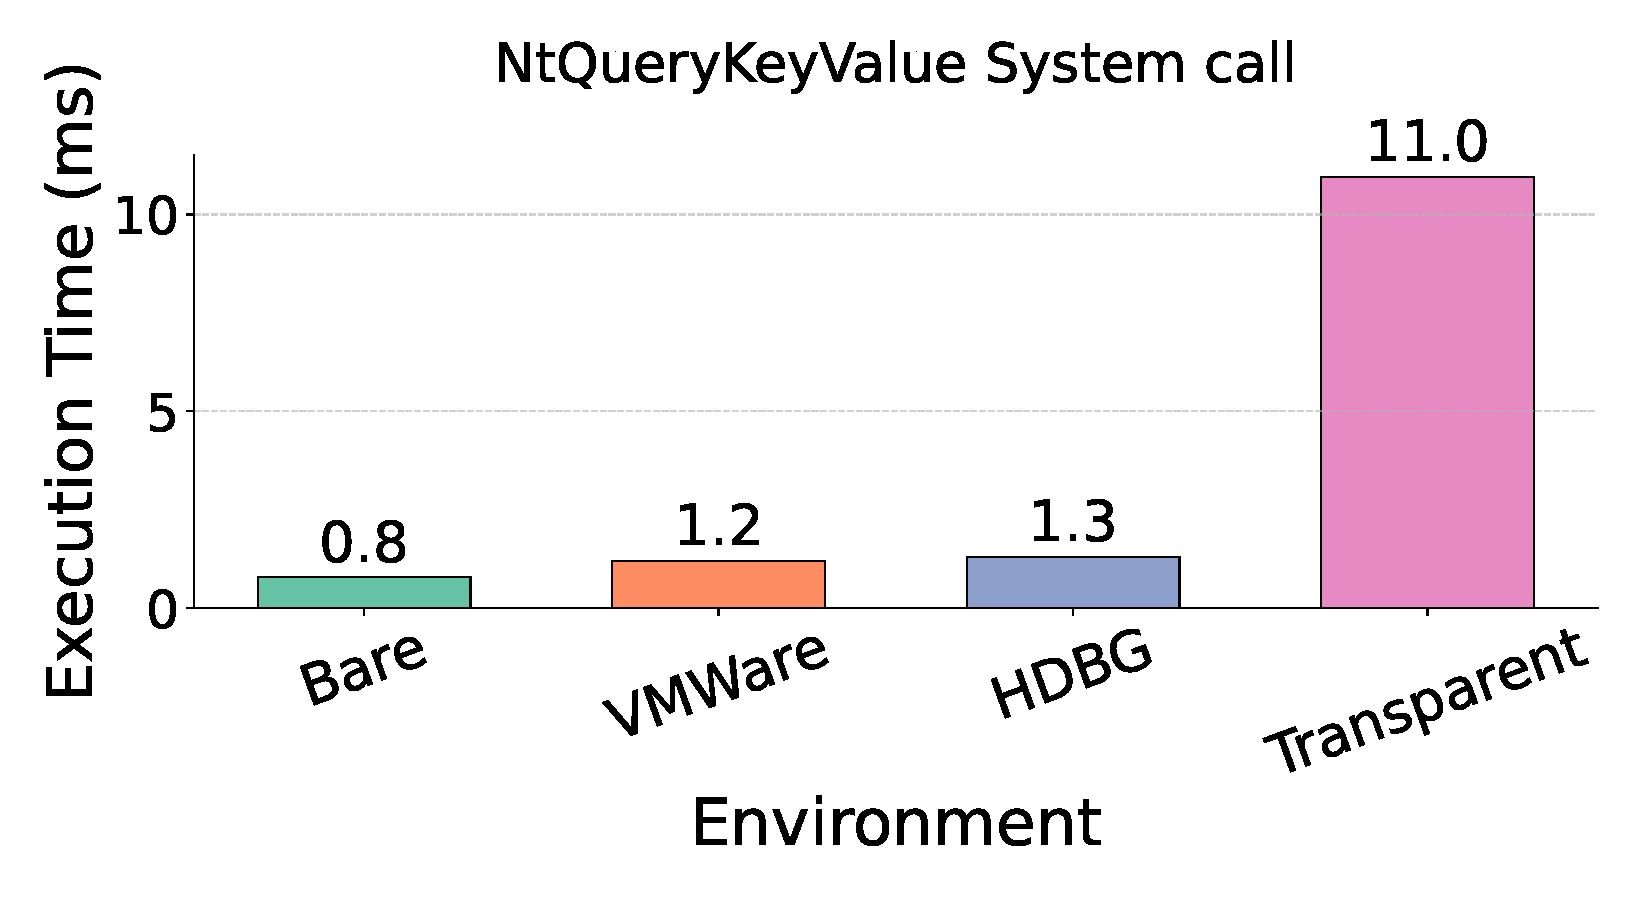
\includegraphics[width=\linewidth]{QKV execution}
        \sfigcap{}\label{fig:exec-time-b}
    \end{subfigure}
    \begin{subfigure}[t]{\threecolgrid}
        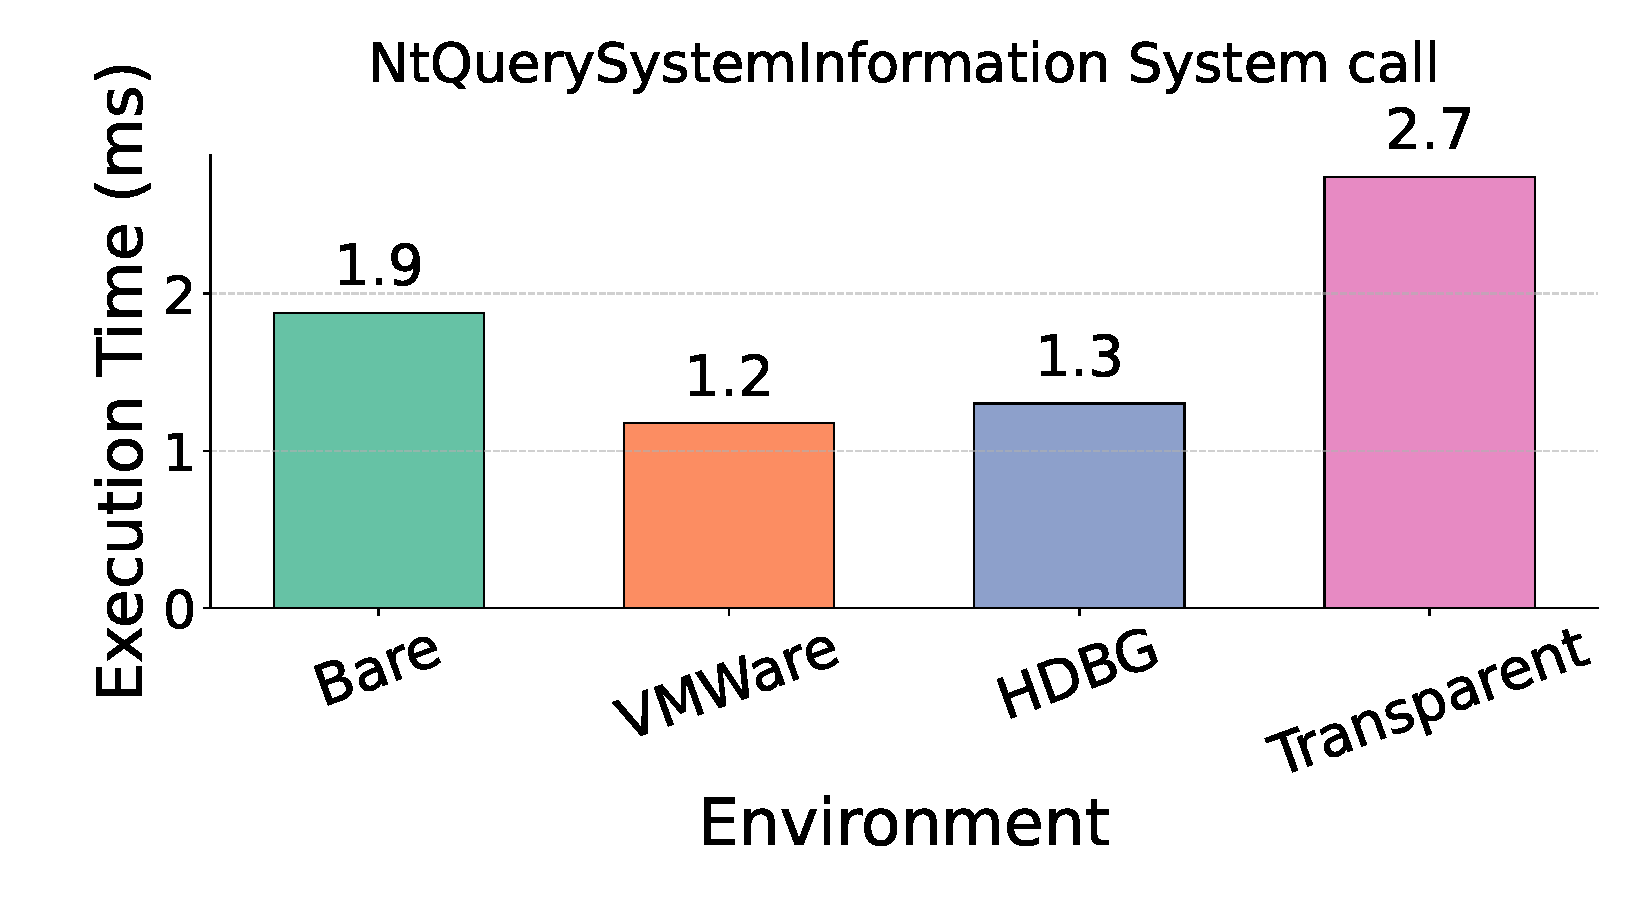
\includegraphics[width=\linewidth]{QSI execution}
        \sfigcap{}\label{fig:exec-time-c}
    \end{subfigure}
    \figcap{Execution time of Windows system calls in different environments. HyperDbg is shortened to \stress{HDBG}, and the data for the detection mitigation transparency mode is labeled as \stress{Transparent}.}\label{fig:execution_time}
\end{figure*}

The real performance impact can be seen in system call interception~\ref{fig:execution_time}. In graph~\ref{fig:exec-time-c} 
the measurements were taken for the NtSystemDebugControl system call. 
This is used by Microsoft debuggers, but can also be used to detect them, including HyperDbg. The transparency mode intercepts this call 
and changes its return value to an error code. A large increase in overhead can also be seen for the NtQueryKeyValue system call~\ref{fig:exec-time-a}, 
for a query of a registry key that would contain hypervisor specific data in its value, if it is read on a virtualized system.
Here the change in execution time is not as large, only 746\% versus the 1240\% increase for NtSystemDebugControl, but the average execution time is a lot longer, in general.

Interestingly, the execution of NtQuerySystemInformation, with a query for the SystemProcessInformation class, reveals less overhead that the other system calls, 
with only a 70\% increase. The lack of more noticeable overhead is because the mitigation for this specific query(\stress{SystemProcessInformation}) 
only requires reading and modifying a user-space memory buffer after the kernel has executed the SYSRET instruction. In contrast, mitigations for NtQueryKeyValue 
also require reading a user-space buffer before the kernel execution, to check the name of the registry key queried. 
The reason for the longer average execution time on the bare metal system is the increased active process count when the tests were performed, increasing the write times in the kernel.

From the intercepted system calls within the transparency mode, NtSystemDebugControl has the smallest code overhead. 
The handler only sets the trap flag for the callback function, in which only the return value in RAX is changed. 
This allows measuring just the overhead introduced by the 2 VM-exits plus the setting of the trap flag, which all the intercepted system call handlers perform. 
With a small error, the transparency overhead visible in graph~\ref{fig:exec-time-a}, is primarily this base overhead introduced by the EPT hook and trap flag VM-exit handlers. 
All system calls handled in the transparency mode will have this base time as the minimum overhead, with additional time delays introduced by memory reads, writes 
as well as any other logic executed in the handler functions.

The time overhead introduced by intercepting the system calls can be measured by malware or any other process in a similar way to how the VM-exit overhead is measured~\ref{HV_detection}. 
This is an issue that needs to be taken into consideration when the hypervisor detection methods are applied to malware analysis or any other process disassembly.

\subsection{Hypervisor Detection}\label{HV-detection-eval}
For the evaluation of the efficiency of the developed hypervisor transparency system, HyperDbg with the transparency mode enabled was deployed against tools that perform many of 
the common hypervisor and debugger detections tests. As a metric, the percentage of positive tests for each tool was measured and compared against running them on HyperDbg 
without the mitigations enabled. These tests were also run on a bare metal system for a base level and false positive measurement. 
The tools chosen for this evaluation were VMAware~\cite{vmaware}, Pafish~\cite{pafish}, and Al-khaser~\cite{al-khaser}, all of them perform numerous known hypervisor and debugger detection methods, 
most of which are also commonly used in malware. At the time of writing this thesis, all 3 are still actively maintained and contain up-to-date detection methods.

Firstly, all of the tools were run on a bare metal machine to test for a base level and detect any false positives that might appear later on. 
Both VMAware and Pafish had 0 positive detections, but Al-khaser showed 1 false positive detection for the Local Descriptor Table(LDT) location test, 
so for the further tests in the virtualized environments, this test was disabled.

Running the testing suites on a VMWare guest system with HyperDbg deployed, but without the transparent mitigations enabled, yielded 16/111 positive detections or 14.41\%, 
Pafish tested 9/58(15.52\%) positive and running Al-khaser resulted in 48/327 positive tests or 14.67, Figure~\ref{fig:test_accuracy}.
It should be noted that many of the tests from all three tools are checking for presence of common consumer virtual machine providers like VMWare and VirtualBox signatures, 
so a lot of the tests performed use the same detection technique, just with different parameters, or searched strings, for these kinds of tests only the VMWare related ones could potentially get a positive score. 
The transparency mode was then enabled, and the same 3 hypervisor detection tools were run. VMAware positively detected only 10/111 (9.01\%) techniques, Pafish caught 6/58 (10.34\%) detection methods, and 
Al-khaser detected the hypervisor in 30 out of 327 attempts, which is 9.17\%, Figure~\ref{fig:test_accuracy}.
\begin{figure}[tbh]
    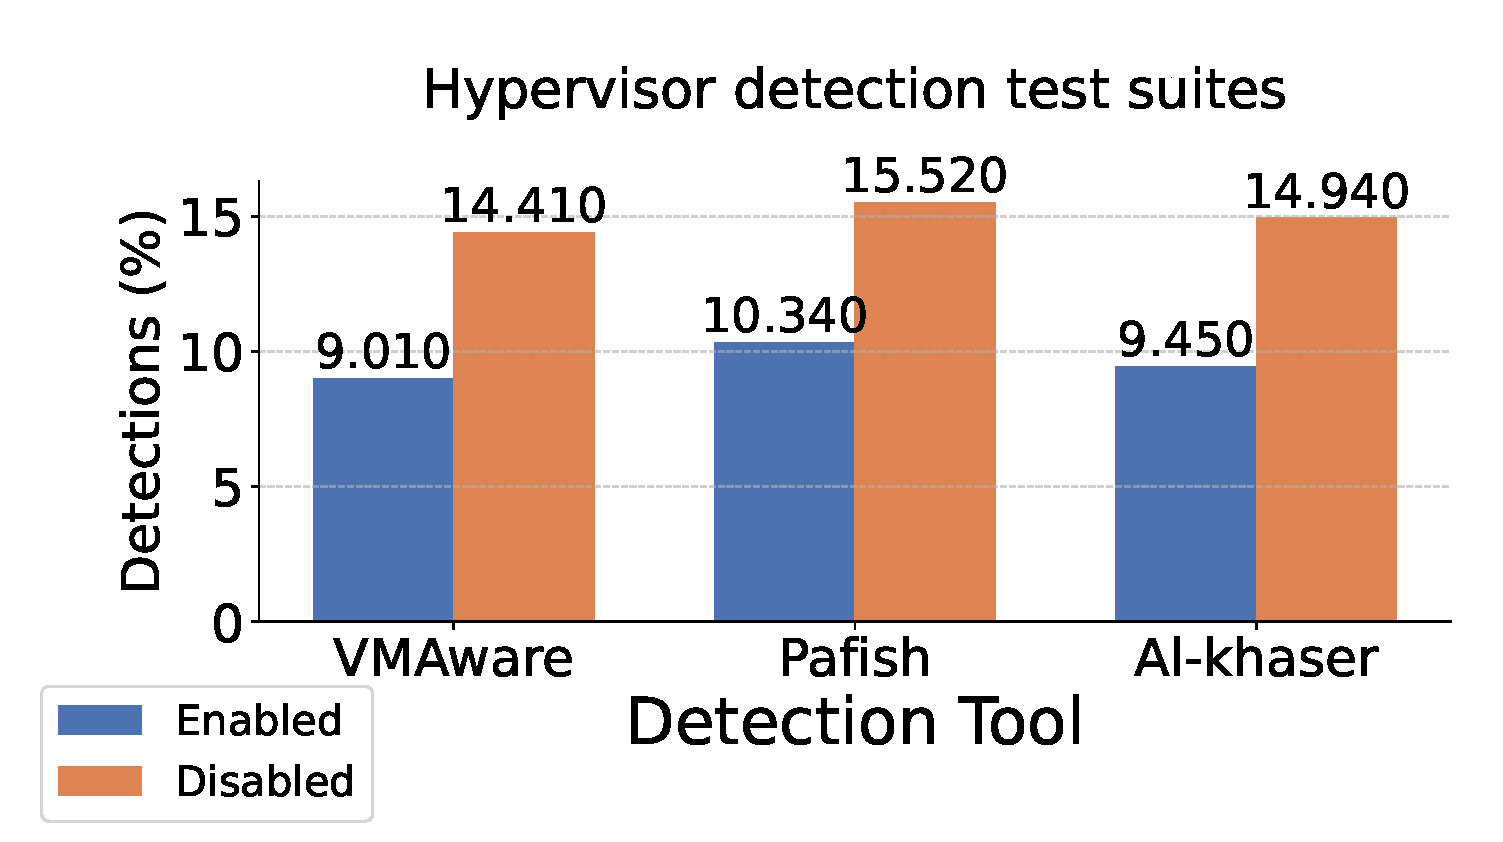
\includegraphics[width=\onecolgrid]{Accuracy tools} %RDTSC_execution
    \figcap{Percentage of positive detections from 3 hypervisor detection suites. \stress{"Enabled"} and \stress{"Disabled"} refer to the transparency mode of HyperDbg being enabled or not during the tests.}\label{fig:test_accuracy}
\end{figure}

Overall, the hypervisor detection mitigation system designed during this project yielded a 37.47\%, 33.38\% and 36.75\% improvement in transparency, 
with a 35.87\% overall average. These test suites primarily tested the system call approach to hypervisor detection and used many of the system calls that had handlers implemented as part of this thesis, 
all of these test methods were successfully mitigated. But since this thesis only tackled a small number of Windows system calls, there were still some detection vectors that had not been intercepted, 
as an example, the system firmware information available from reading a certain registry key\footnote{Information on firmware data available in the Windows registry. Microsoft. \url{https://learn.microsoft.com/en-us/windows-hardware/drivers/install/registry-trees-and-keys}} 
or from NtQuerySystemInformation with the SystemFirmwareTableInformation class. This structure was chosen not to be intercepted, and so, 
an attempt to read it from a virtualized system would still reveal hypervisor presence.

Evaluating the efficiency of the transparency features revealed the minimal instability in the implementation. The source of the system instability 
could not be definitively identified, but it caused only rare system crashes, and could not be measured.


\subsection{Comparison with ScyllaHide}\label{scyllahide-comparison}
HyperDbg is not just a hypervisor, it is also a kernel-space debugger~\cite{karvandi2022hyperdbg}. This means that during the design of 
the hypervisor transparency features, mitigating debugger detections was also taken into consideration. The approach of intercepting Windows system calls 
from the kernel-space allows HyperDbg to stay undetectable from any user-space process. ScyllaHide is a tool for debugger detection mitigation~\cite{scyllahide}, 
which stays in the user-space, and while it can mitigate most attempts at detecting a kernel-space debugger, ScyllaHide can only intercept API calls at the user-space level. 
This could allow detection attempts to bypass ScyllaHide by calling specific Windows system calls directly, avoiding the NT API interception. 

In the design proposed in this thesis, the system call interception resides at the kernel level (ring 0), with the mitigations performed at ring -1, 
so even the direct system call invocation would be mitigated. To test this, a simple C++ program was created that called a specific Windows system call, 
NtSystemDebugControl. Firstly, using the NT API wrapper function with the same name and then directly, by emulating the API wrapper function.
\begin{listing}[!ht]

\begin{minted}[linenos,frame=single]{nasm}
    MOV R10, RCX
    MOV EAX, 0x01D0 ; System call number
    SYSCALL
    RET
\end{minted}
\caption{Windows system call wrapper function for NtSystemDebugControl from the NTDLL library.}
\label{lst:syscall-wrapper}
\end{listing}
When ScyllaHide was deployed and attached to the process of the created testing program, only the API call version could be intercepted and mitigated, 
while any tests calling directly to the kernel could bypass the transparent mitigations of ScyllaHide.
On the other hand, when HyperDbg's transparency mode is enabled and deployed on the system. Performing the same tests, both attempts can be intercepted and 
successfully mitigated.



%%% Local Variables:
%%% mode: latex
%%% TeX-master: "../thesis"
%%% End:
